% Chapter 3: State of the Art

\chapter{Estado del Arte} % Main chapter title

\label{Chapter3} % For referencing this chapter elsewhere, use \ref{Chapter2}

%----------------------------------------------------------------------------------------

 \section{Java}

 %----------------------------------------------------------------------------------------

 \section{Android}

 %----------------------------------------------------------------------------------------

 \section{Bouncy Castle}

 Bouncy Castle (BC), también llamado Bouncy Castle Crypto, es una colección de APIs utilizados en criptografía. Tiene versiones para los lenguajes Java y C\#.

 La arquitectura de BC consta de dos componentes principales que soportan las prestaciones básicas de criptografía.
 Estos son una API \emph{ligera} y un proveedor para Java Cryptography Extension (JCE)\footnote{JCE implementa encriptación, generación y protocolos de establecimiento de claves y algoritmos MAC.}.
 Otros componentes basados en el proveedor para JCE admiten funciones adicionales, como soporte para PGP, S/MIME, etc. \emph{\parencite{Reference4}}

 \begin{figure}[ht]
   \centering
   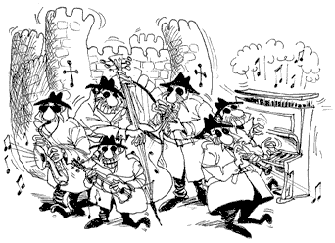
\includegraphics{Figures/BouncyCastle}
   \decoRule
   \caption[Legion of Bouncy Castle]{The Legion of Bouncy Castle, creadores de Bouncy Castle}
   \label{fig:BouncyCastle}
 \end{figure}

 %----------------------------------------------------------------------------------------

 \section{Padding}

 %----------------------------------------------------------------------------------------

 \section{Criptografía de clave pública}

 La criptografía de clave pública, también llamada criptografía asimétrica, es el método criptográfico que usa un par de claves para la firma y el cifrado de mensajes.
 Una clave es \emph{pública} y se puede entregar a cualquier persona, la otra clave es \emph{privada} y el propietario debe guardarla de modo que nadie tenga acceso a ella.

 Si el remitente usa la clave pública del destinatario para cifrar el mensaje, una vez cifrado, sólo la clave privada del destinatario podrá descifrar este mensaje, ya que es el único que la conoce.
 Por tanto se logra la \emph{confidencialidad} del envío del mensaje, nadie salvo el destinatario puede descifrarlo.

 Si el propietario del par de claves usa su clave privada para cifrar el mensaje, cualquiera puede descifrarlo utilizando su clave pública.
 En este caso se consigue por tanto la \emph{identificación} y \emph{autentificación} del remitente, ya que se sabe que sólo pudo haber sido él quien empleó su clave privada (salvo que alguien se la hubiese podido robar).
 Esta idea es el fundamento de la firma electrónica\footnote{Existen multitud de algoritmos de firma, para este proyecto se ha optado por usar RSASSA-PSS}. \emph{\parencite{Reference5}}

 \begin{figure}[ht]
   \centering
   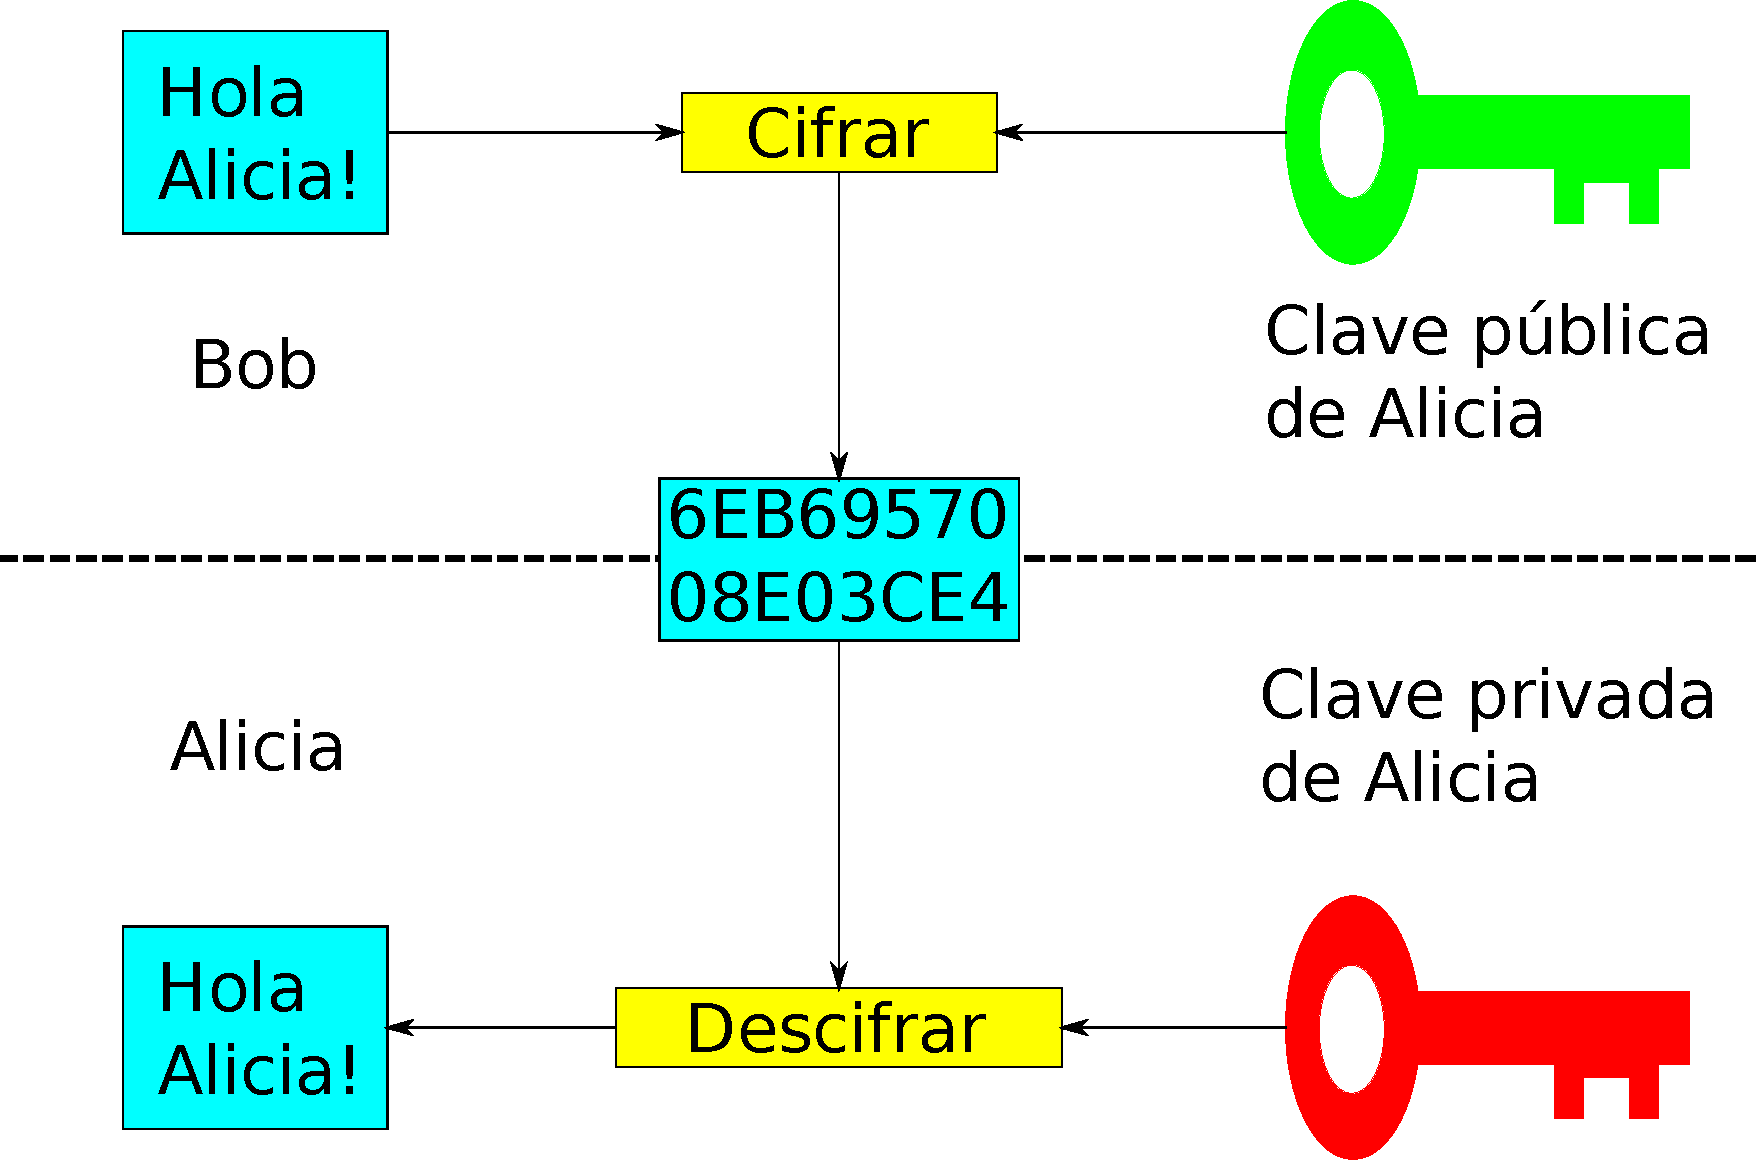
\includegraphics[scale=0.5]{Figures/PublicKeyEncryption}
   \decoRule
   \caption[Cifrado de clave pública]{Esquema general del cifrado de clave pública}
   \label{fig:PublicKeyEncryption}
 \end{figure}

 %----------------------------------------------------------------------------------------

 \section{RSA}

 %----------------------------------------------------------------------------------------

 \section{RSASSA-PSS}

 %----------------------------------------------------------------------------------------

 \section{Criptografía de clave simétrica}

 %----------------------------------------------------------------------------------------

 \section{Cifrado de bloques}

 %----------------------------------------------------------------------------------------

 \section{CBC}

 %----------------------------------------------------------------------------------------

 \section{AES}

 %----------------------------------------------------------------------------------------

 \section{HTTP}
